\subsubsection{Overview}


\begin{figure}
\centering
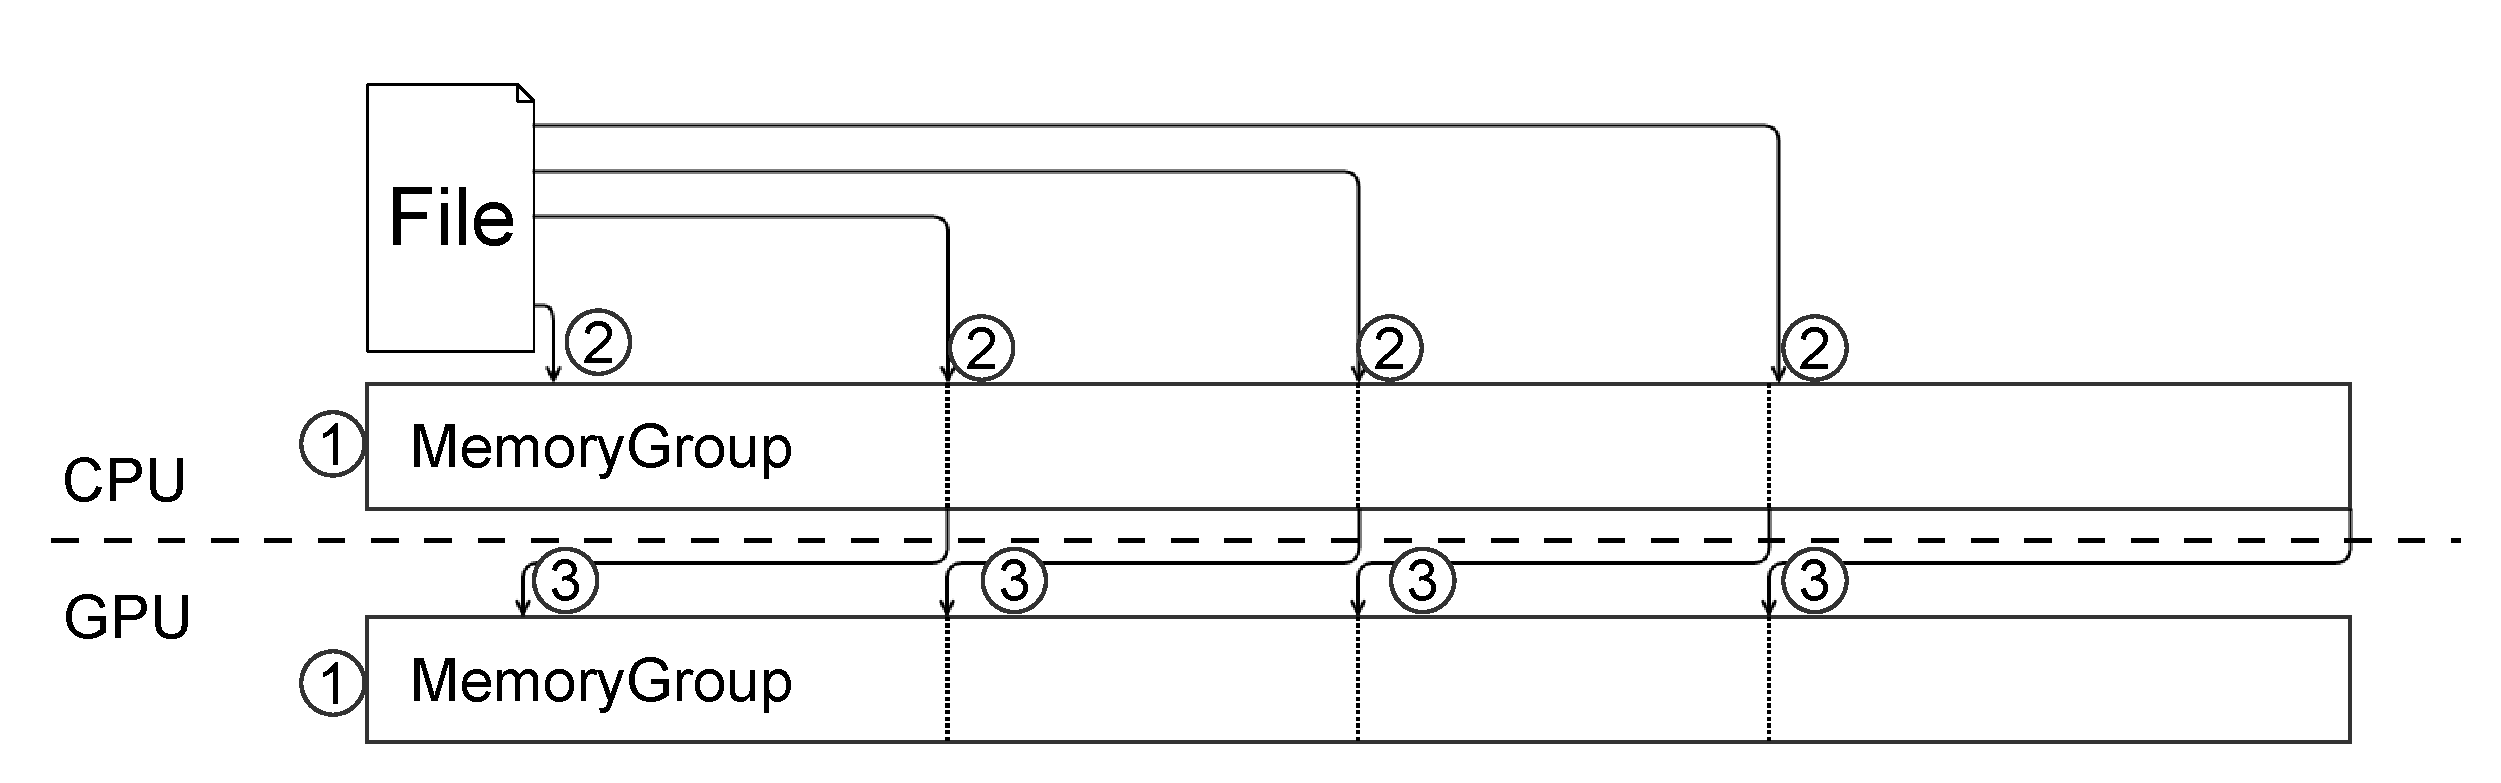
\includegraphics[scale=0.2]{fig/memory_group.pdf}
\caption{Memory Streaming Design}
\label{fig:memorygroup}
\centering
\end{figure}

The runtime simplifies our code generator by abstracting common operations
	into (essentially) a separate project.
The runtime's job is to eagerly copy data to the GPU and execute the
 	computation while maintaining the dependencies.

To unify memory, we define a new object called a \fix{zMemoryGroup\_t}
This object contains multiple \fix{zMemory\_t}s which,
	index into a contiguious array buffer for both CPU and GPU memories.
Each \fix{zMemory\_t} has a status, such as
	\fix{unalloacted}, \fix{allocated},
	\fix{dirtyDevice}, etc\ldots
	that allow us to maintain conherence and avoid copies when
	not necessary.
The memory object also contains size and type information,
	and the runtime operates on \fix{zMemory\_t} rather than \fix{void *}
	types.
This abstraction will eases adding support for other languages, such
	as OpenCL, without changing the code generator.

To eagerly copy memory to the GPU, we use logic similar to what is
	shown in Figure~\ref{fig:memorygroup}.
In (1), we concurrently alloate CPU memory and GPU memory.
The file is then opened in (2) and different chunks are read into
	the CPU memory one it's been allocated (we \fix{mmap} the file
	with the \fix{PROT\_READ} and \fix{MAP\_PRIVATE} options to increase
	performance).
Once a chunk of data is read and the GPU memory has been allocated, data
	is copied to the GPU in (3).
Note that while we have an abstracted view of chunks of memory
	(defined by the datatype \fix{zMemory\_t}), memory is in fact
	contiguious and placed in a \fix{zMemoryGroup\_t} object.
This makes it possible to resize and free memory efficiently.
